\documentclass[a4paper, 12pt]{report}

\usepackage{charter}
\usepackage{makeidx}
\usepackage{fancyhdr}
\usepackage{hyperref}
\usepackage[utf8]{inputenc}
\usepackage{graphicx}
\usepackage[left=2cm, right=2cm]{geometry}
\usepackage{latexsym}
\usepackage{amsmath, amsthm, amssymb}
\usepackage{rotating}



\begin{titlepage}
\title{Piano dei tests}
\author{Release 0.6}
\date{\today \\Firenze \\\begin{figure}[h] \centering 

\includegraphics[width=0.2\textwidth]{../images/logokiwi.png} \end{figure} }
\end{titlepage}

\newtheorem{taksDef}{Definizione}[subsection]

\pagestyle{fancy}
 
\begin{document}

\maketitle

\section*{Approvazione, redazione, lista distribuzione}
\begin{table}[h!]
  \begin{center}
    \begin{tabular}{| l | l | p{60mm} |}
    \hline
    \textbf{approvato da} & \textbf{il giorno} & \textbf{firma} \\
	\hline    
	Marco Tinacci & \today &  \\
    \hline
    \end{tabular}
  \end{center}
\end{table}

\begin{table}[h!]
  \begin{center}
    \begin{tabular}{| l | l | p{60mm} |}
    \hline
    \textbf{redatto da} & \textbf{il giorno} & \textbf{firma} \\
	\hline    
	Manuele Paulantonio & \today &  \\
    \hline
	Daniele Poggi & \today &  \\
    \hline
	Massimo Nocentini & \today &  \\
    \hline
    \end{tabular}
  \end{center}
\end{table}

\begin{table}[h!]
  \begin{center}
    \begin{tabular}{| l | l | p{60mm} |}
    \hline
    \textbf{distribuito a} & \textbf{il giorno} & \textbf{firma} \\
	\hline    
	Francesco Calabri & \today &  \\
    \hline
	Niccol\'o Rogai & \today &  \\
    \hline
	Marco Tinacci & \today &  \\
    \hline
    \end{tabular}
  \end{center}
\end{table}

\tableofcontents

\part{Planning}

\chapter{Master Plan}
\section{Scope}

Questo \`e il \emph{Master Plan} per il progetto \textbf{PMango}. Questo piano
considera solo gli elementi software relativi alle aggiunte/modifiche descritte
nel documento di analisi. \\ \\
L'obiettivo primario di questo piano di test \`e quello di assicurare che la
nuova versione di \textbf{PMango} offrir\`a lo stesso livello di informazioni e
dettagli reso disponibile della versione corrente e aggiunger\`a tutte quelle
informazioni necessarie per raggiungere gli obiettivi modellati dal processo di
analisi.
\\ \\
Il progetto avr\`a tre livelli di testing: 
\begin{itemize}
  \item unit
  \item system/integration
  \item acceptance
\end{itemize}
I dettagli di ogni livello verranno definiti nella sezione \ref{subsec:strategy}
e negli specifici \emph{level plan}. \\ \\
Il quanto temporale stimato per questo progetto \`e molto compatto, quindi
\emph{ogni} ritardo nella fase di progettazione, sviluppo, installazione e
verifica possono avere effetti significati sul deploy finale.

\section{Elementi software sottoposti a test}

\begin{itemize}
  \item some components produced by the detailed desing team
\end{itemize}

\section{Funzionalit\`a che verranno testate}
\begin{itemize}
  \item processo per la generazione di \emph{Gantt chart}
  \item processo per la generazione di \emph{WBS chart}
  \item processo per la generazione di \emph{Task Network chart}
  \item interfaccia grafica per la selezione delle nuove \emph{UserOption} per
  ogni \emph{Chart}
  \item aggiunta di ogni \emph{Chart} alla sezione di reportistica
\end{itemize}

\section{Software Risk Issues}
Ci sono alcuni punti che ci portano a definire questa sezione:
\begin{itemize}
  \item Reverse engineering di codice sorgente esistente, documentato nei sorgenti
ma non ha documenti ufficiali (apparte le tesi) che descrivino in modo chiaro
la struttura statica e dinamica di tutto il lavoro esistente.
  \item Uso di librerie esterne per la generazione delle immagini e dei
  documenti pdf.
\end{itemize}

\section{Strategia}

\subsection{Testing machines}
Identifichiamo due classi di macchine sulle quali viene condotto il processo di
testing:
\begin{itemize}
  \item \emph{develop machine} macchine dove avviene sia lo sviluppo del codice
  che parte del testing.
  \item \emph{acceptance machine} macchine (molto probabilmente unica, a meno
  di guasti) dove avviene solo il processo di testing.
\end{itemize}

\subsection{Strumenti}
\label{subsec:testingTools}
Durante il processo di testing usufruiamo dei seguenti strumenti:
\begin{itemize}
  \item controllo visivo umano per quanto riguarda il confronto dell'output
  con l'output atteso (descritto nei documenti \emph{Test case specification})
  per quanto riguarda immagini
  \item utilizzo di verifica automatica di batterie di test usando l'insieme di
  oggetti contenuti nella distribuzione di \emph{phpUnit} oppure attraverso
  classi di test non appartenenti al precedente framework ma che hanno la
  stessa idea di verifica (controllo automatico tra output e risultato
  previsto).
\end{itemize}

\subsection{Test failure's metrics}
Modelliamo il concetto di \emph{failure} aggiungendo delle informazioni, in
modo da specializzarlo per il nostro processo di testing. Ogni
specializzazione ha il significato di esprimere la gravit\`a (importanza) del
fallimento. Quindi, l'esito di un test pu\`o essere \emph{success} o
\emph{failure}, nel secondo caso aggiungiamo queste specializzazioni:
\begin{description}
  \item[minor] il fallimento del test non \`e da considerarsi un evento grave.\\
  Gli oggetti software che hanno prodotto questa failure possono essere comunque
  inseriti nella release di \textbf{PMango 3}, non impediscono l'avanzare dello
  sviluppo. Possiamo identificare di questa failure come un \emph{defect}.
  \item[critical] il fallimento del test \`e da considerarsi un evento grave.\\
  Gli oggetti software che hanno prodotto questa failure non possono essere
  inseriti nella release di \textbf{PMango 3}, necessitano di ricontrollare il
  codice relativo a tali oggetti; non impediscono l'avanzare dello sviluppo.
  \item[blocking] il fallimento del test \`e da considerarsi un evento grave.\\
  Gli oggetti software che hanno prodotto questa failure non possono essere
  inseriti nella release di \textbf{PMango 3}, necessitano di ricontrollare il
  codice relativo a tali oggetti e, se necessario, ricontrollare il relativo
  documento di progettazione; impediscono l'avanzare dello sviluppo.
\end{description}
Queste misure sono valide per tutte le failure di test appartenenti a ogni
level plan descritto in \ref{sec:levelPlans}.


\section{Level plans}
\label{sec:levelPlans}
\subsection{Definitions}
\label{subsec:strategy}
Il processo di testing per il progetto \textbf{PMango} consiste nei livelli
seguenti.
\begin{description} 
\item[unit] questo livello viene effettuato da tutti gli
sviluppatori e stilato dal team dei verificatori con un rapprensentante degli
sviluppatori. 
\\ \\
Ogni motivazione riguardo ogni singolo unit test deve essere resa disponibile e
documentata in modo chiaro o in un documento apposito\footnote{inserire un
riferimento al relativo documento di test case specification} oppure nel codice
nel caso che 
\begin{itemize}
	\item viene utilizzato un strumento automatico indicato nelle sezione
	\ref{subsec:testingTools}
	\item la motivazione ha una dimensione ragionevolmente corta che \`e
	possibile inserirla come commento nel codice 
\end{itemize}

Questo livello viene esercitato su macchine di tipo \emph{develop machine}.

\item[system/integration] questo livello viene eseguito dal
team dei verificatori in presenza di un rappresentante degli sviluppatori
se necessario. 
\\ \\
Ogni motivazione e descrizione di questi test deve essere esposta nei documenti
\emph{Test case specification}
\\ \\
Questo livello viene esercitato su macchine di tipo \emph{acceptance machine} e
\emph{develop machine}.

\item[acceptance] questo livello viene eseguito dal cliente in presenza di un
rapprensentante dei verificatori.
\\ \\
Una volta terminato il livello di \emph{acceptance} il prodotto viene
rilasciato al cliente il quale pu\`o continuare la fase di testing in parallelo
alla fase di utilizzo.
\\ \\
Questo livello viene esercitato su macchine di tipo \emph{develop machine}.

\end{description}

\subsection{Precedence Relation}
Possiamo costruire la relazione di precedenza $\sqsubset$ fra coppie di level
plan che permette ad un oggetto software di avanzare nel processo di testing,
in modo da garantire il suo corretto funzionamento durante la fase di
revisione congiunta oppure nel collaudo. 

Definiamo $\sqsubset$ in questo modo: 
\begin{description}
  \item[unit $\sqsubset$ system/integration] ogni oggetto software entra nel 
processo di testing dal level plan \emph{unit}. 

Quando soddisfa tutti i suoi \emph{unit} test oppure, per ogni fallimento, la
metrica misura \emph{minor}, allora pu\`o essere disponibile per il level plan 
\emph{system/integration} se \`e richiesto da qualche \emph{system/integration}
test.
  \item[system/integration $\sqsubset$ acceptance] quando un oggetto (o gruppo
  di oggetti) superano tutti i test oppure, per ogni fallimento, la metrica 
  misura \emph{minor}, allora l'oggetto (o gruppo di oggetti) pu\`o avanzare
  nel level plan \emph{acceptance}
\end{description}
La relazione $\sqsubset$ \`e riflessiva, in quanto un test permane in un level
plan finche non soddisfa i requisiti per passare nel successivo; non \`e ne
simmetrica ne transitiva, in quanto vogliamo garantire al committente la
sequenzialit\`a del processo di testing.

Osservazione: quando un test passa da un livello al successivo deve essere
continuo rispetto alla batteria dei test specificata nel livello che lascia.
Ovvero: se avanza di livello deve continuare a soddisfare le condizioni che gli
hanno permesso di avanzare fino al livello corrente.



\section{Pass/fail criteria}
Il risultato dell'intero piano delle prove \`e dato dalla seguente relazione:
\begin{table}[h!]
  \begin{center}
    \begin{tabular}{| l | l |}
    \hline
    \textbf{risultato} & \textbf{criteri} \\
	\hline    
	success & numero di \emph{minor} failures $\leq 10$   \\
    \hline
    \emph{minor} failure & numero di \emph{minor} failures $> 10$ \\
    \hline
    \emph{critical} failure & almeno una \emph{critical} failure \\
    \hline
    \emph{blocking} failure & almeno una \emph{blocking} failure \\
    \hline
    \end{tabular}
  \end{center}
	\caption{La colonna \emph{criteri} si riferisce all'insieme dei \emph{design
	specification} definite in \ref{part:DesignSpecification}}
\end{table}

Il processo di testing verr\`a completato nella data in cui avverr\`a il
collaudo con il committente oppure quando questo piano da esito
\emph{success} in base alla relazione definita dalla tabella, prima del
collaudo. Dalla fine del processo di testing, la nuova versione di PMango
viene considerata \emph{live}. \\ \\ 
Nel caso in cui il nostro team non riuscisse a portare a termini gli impegni 
presi entro la data del collaudo, il processo di testing proseguir\`a fino alla
data in cui si considera terminato il tempo a disposizione per eseguire l'esame.

\section{Enviromental needs}
I seguenti elementi sono richiesti per supportare l'intero processo di testing:
\begin{itemize}
  \item Sia \emph{develop machine} che \emph{acceptance machine} devono avere
  installato una istanza di un server (L/W/M)AMP, con tutti i necessari permessi
  per la corretto funzionamento, relativamente al sistema operativo presente
  \item Sia \emph{develop machine} che \emph{acceptance machine} devono offrire
  tutte quelle \emph{third party resources} necessarie per l'utilizzo della
  nuova versione di PMango (fonts microsoft, \ldots) compresi tutte quelle
  necessarie per la versione di PMango attuale.
\end{itemize}


\part{Desing Specification}
\label{part:DesignSpecification}
\chapter{Generate Chart Design}
\section{Features to be tested}
\label{sec:GenerateChart}
\begin{figure}[h!] 
\centering 
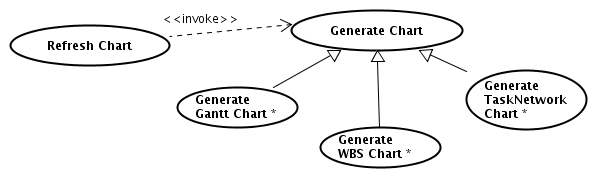
\includegraphics[width=0.7\textwidth]{desing_spec/GenerateChart.png}
\caption{spaccato tratto dal package \emph{Commons} del documento di analisi,
parte \emph{Use cases}}

\end{figure}
Verranno testati tutti gli use case espressi dalla figura tranne ``Refresh
Chart'' in quanto \`e stato riportato solo per favorire la comprensione del
contesto e perche la sua attivit\`a di costruire la \emph{UserOptionChoice} e
recuperare l'insieme dei \emph{Task} vengono testate nel documento
\footnote{make a test document for these use cases.}

\section{Raffinamento della strategia}
\begin{description}
  \item[costruzione strutture di input] Gli usi case descritti nella sezione 
\ref{sec:GenerateChart}, verranno testati usando come input strutture valide e
strutture non valide. Le strutture di input (sia valide che non) verranno
definite in modo che lo use case venga esercitato per la generazione dei
dettagli descritti nel documento di analisi e cercare di provare la generazione
di gran parte delle notazioni grafiche (relative al tipo \emph{Chart} che si
sta considerando).
  \item[confronto dell'output] Per ogni use case di ``generazione'' verranno 
  prodotti dei modelli, in notazione \emph{mockup} disegnati a mano, per poter 
  effettuare il confronto con le immagini di output generate
  dall'implementazione.
  \item[modalit\`a di esecuzione] Ogni use case verr\`a esercitato in modo 
  \emph{individuale}, non verranno esercitate combinazioni con altri use case,
  come la figura esprime.
\end{description}

\section{Tests identification}
\label{sec:GenerateChartTestIdentification}
Sotto vi sono i reference a tutte le \emph{case specification} relative a
questo \emph{desing}, definite in \ref{part:CaseSpecification}:
\begin{itemize}
  \item \nameref{chap:generateGantt}
  \item \nameref{chap:generateWBS}
  \item \nameref{chap:generateTaskNetwork}
\end{itemize}

\section{Pass/fail criteria}
Il risultato di questo desing \`e
espresso dalla seguente relazione rappresentata da questa tabella: 
\begin{table}[h!]
  \begin{center}
    \begin{tabular}{| l | l |}
    \hline
    \textbf{risultato} & \textbf{criteri} \\
	\hline    
	success & numero di \emph{minor} failures $\leq 5$   \\
    \hline
    \emph{minor} failure & numero di \emph{minor} failures $> 5$ \\
    \hline
    \emph{critical} failure & almeno una \emph{critical} failure \\
    \hline
    \emph{blocking} failure & almeno una \emph{blocking} failure \\
    \hline
    \end{tabular}
  \end{center}
	\caption{La colonna \emph{criteri} si riferisce all'insieme di tests 
	identificati nella sezione \ref{sec:GenerateChartTestIdentification}}
\end{table}


\part{Case Specification}
\label{part:CaseSpecification}
\chapter{Generate Chart - Invalid input}
\label{chap:genChartInvInput}

\section{Input}
\label{sec:generateGanttInvalidInput}
\subsection{Project plan}
\begin{figure}[h!] 
\centering
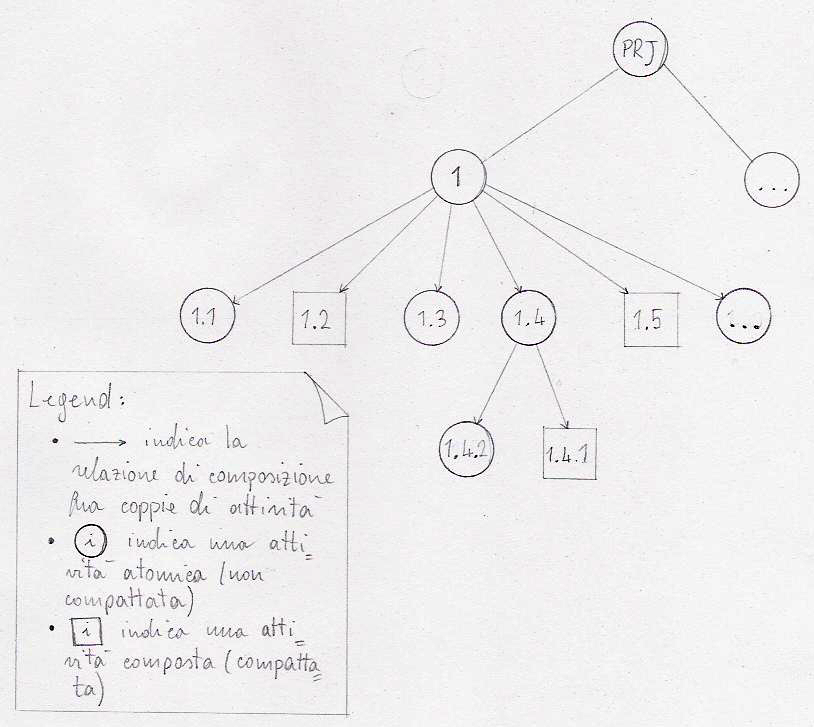
\includegraphics[width=0.6\textwidth]{case_spec/generate_Gantt/invalidInput.png}
\caption{invalid input structure}
\end{figure}

\subsection{Task definitions}
\begin{taksDef}{Task 1.4.1} \`E un task composto e la visualizzazione che si
vuole \`e di vederlo compattato; si valorizzano le propriet\`a:
\begin{itemize}
  \item $Name = ``Trasporti"$
  \item $StartDate_{planned} = 06/11/2009$
  \item $FinishDate_{planned} = 11/11/2009$
  \item $StartDate_{actual} = 07/11/2009$
  \item $FinishDate_{actual} = 12/11/2009$
\end{itemize}
\end{taksDef}

\begin{taksDef}{Task 1.4.2} \`E un task atomico; si valorizzano le propriet\`a:
\begin{itemize}
  \item $Name = ``Ordinazioni"$
  \item $StartDate_{planned} = 09/11/2009$
  \item $FinishDate_{planned} = 16/11/2009$
  \item $StartDate_{actual} = 10/11/2009$
  \item $FinishDate_{actual} = 11/11/2009$
\end{itemize}
\end{taksDef}

\begin{taksDef}{Task 1.4} \`E un task composto e si vuole visualizzare i task che lo
compongono; si valorizzano le propriet\`a:
\begin{itemize}
  \item $Name = ``Mense"$
  \item $StartDate_{planned} = 06/11/2009$
  \item $FinishDate_{planned} = 16/11/2009$
  \item $StartDate_{actual} = 07/11/2009$
  \item $FinishDate_{actual} = 12/11/2009$
\end{itemize}
\end{taksDef}

\begin{taksDef}{Task 1.1} \`E un task atomico
; si valorizzano le propriet\`a:
\begin{itemize}
  \item $Name = ``Allocazione"$
  \item $StartDate_{planned} = 02/11/2009$
  \item $FinishDate_{planned} = 06/11/2009$
  \item $StartDate_{actual} = 30/10/2009$
  \item $FinishDate_{actual} = 04/11/2009$
\end{itemize}
\end{taksDef}

\begin{taksDef}{Task 1.2} \`E un task composto; si valorizzano le propriet\`a:
\begin{itemize}
  \item $Name = ``Gestione\quad cibo"$
  \item $StartDate_{planned} = 04/11/2009$
  \item $FinishDate_{planned} = 10/11/2009$
  \item $StartDate_{actual} = 13/11/2009$
  \item $FinishDate_{actual} = 17/11/2009$
\end{itemize}
\end{taksDef}

\begin{taksDef}{Task 1.3} \`E un task atomico; si valorizzano le propriet\`a:
\begin{itemize}
  \item $Name = ``Gestione\quad Fornitori"$
  \item $StartDate_{planned} = 03/11/2009$
  \item $FinishDate_{planned} = 10/11/2009$
  \item $StartDate_{actual} = 13/11/2009$
  \item $FinishDate_{actual} = 17/11/2009$
\end{itemize}
\end{taksDef}

\begin{taksDef}{Task 1.5} \`E un task composto; si valorizzano le
propriet\`a:
\begin{itemize}
  \item $Name = ``Fatturazione"$
  \item $StartDate_{planned} = 18/11/2009$
  \item $FinishDate_{planned} = 21/11/2009$
  \item $StartDate_{actual} = 15/11/2009$
\end{itemize}
\end{taksDef}

\begin{taksDef}{Task 1} \`E un task composto; si valorizzano le propriet\`a:
\begin{itemize}
  \item $Name = ``Progetto\quad pasti"$
  \item $StartDate_{planned} = 02/11/2009$
  \item $FinishDate_{planned} = 21/11/2009$
  \item $StartDate_{actual} = 30/10/2009$
\end{itemize}
\end{taksDef}

\subsection{Task dependencies}
Possiamo creare la relazione $\sqsubset$ \emph{FinishToStart} che associa due
task in questo modo:
\begin{displaymath}
\sqsubset = \lbrace (a,b) : b_{startDate} >= a_{startDate}, \forall a,b \in
DependencyTask
\rbrace
\end{displaymath}
con \emph{DependencyTask} l'insieme di tutti i task creati definendo la
relazione di dipendenza attraverso la relativa pagina di editing disponibile in
PMango. 

Possiamo quindi applicare la definizione di $\sqsubset$ al nostro input:
\begin{displaymath}
\sqsubset = \lbrace (1.2, 1.1), (1.4.2, 1.3), (1.4, 1.5), (1.5, 1.4.2)
\rbrace
\end{displaymath}

\section{Environment}
Si vuole generare l'output con l'istanza di input sepecificata nella sezione
\ref{sec:generateGanttInvalidInput}. Come oggetti appartenti al contesto di
generazione, fissiamo queste \emph{UserOption}:
\begin{description}
  \item[TimeRangeUserOption] valorizza
  \begin{itemize}
  \item $FromStartRange = 26/10/2009$
  \item $ToEndRange = 06/12/2009$
  \end{itemize} 
  \item[TimeGrainUserOption] $= ``DailyGrain''$
  \item[TaskName] = $checked$
  \item[WBSUserSpecificationUserLevel] = $checked$
  \item[ShowDependencies] = $checked$
\end{description}

\section{Output}
\begin{sidewaysfigure}[h!] 
\centering
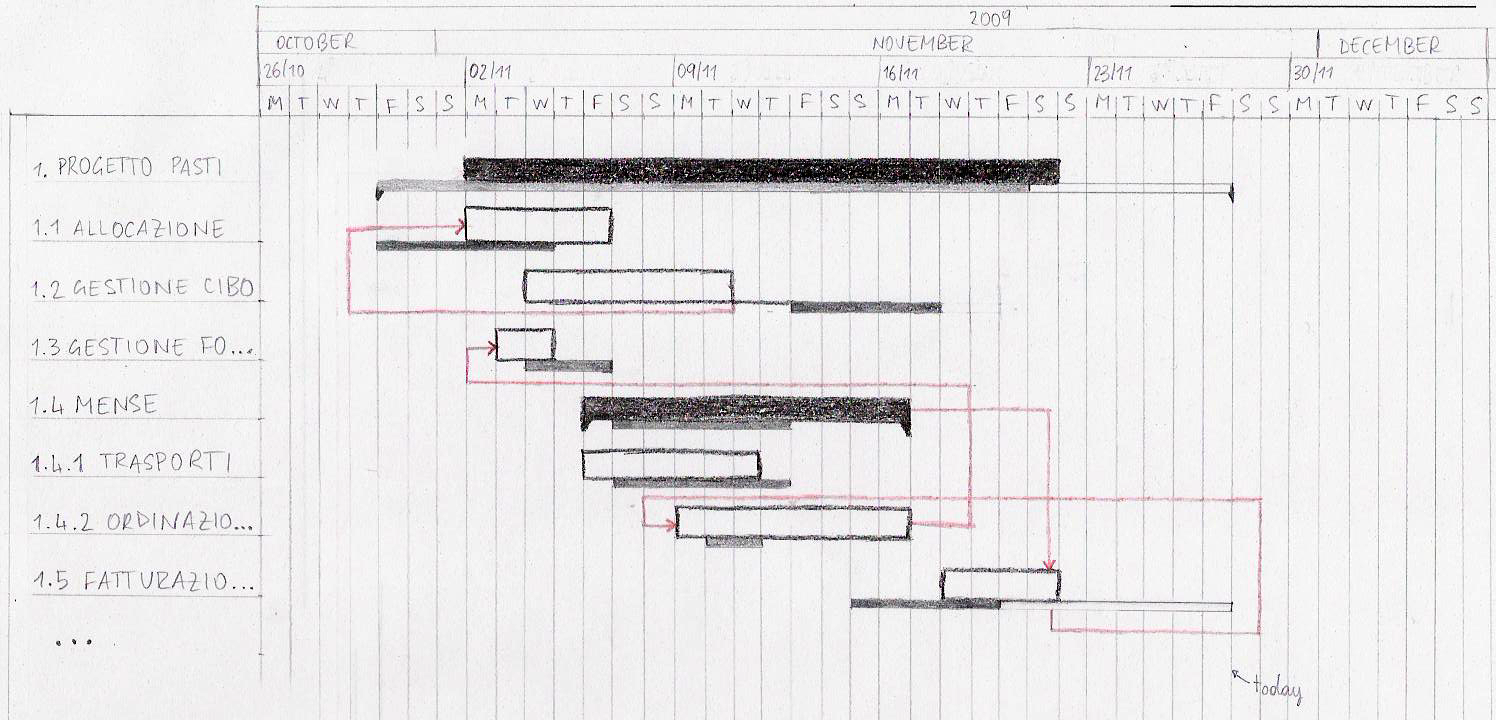
\includegraphics[width=1\textwidth]{case_spec/generate_Gantt/invalidOutput.png}
\caption{output for the invalid input structure}
\label{fig:generateGanttInvalidOutputMockup}
\end{sidewaysfigure}
See figure \ref{fig:generateGanttInvalidOutputMockup}.

\section{Pass/fail criteria}
\begin{table}[h!]
  \begin{center}
    \begin{tabular}{| l | p{100mm} |}
    \hline
    \textbf{risultato} & \textbf{criteri} \\
	\hline    
	success & l'output dell'implementazione \`e sovrapponibile al modello a meno 
di una tolleranza pari a circa \textbf{1mm}. I punti di stacco dei segmenti
delle dipendenze possono disposti in maniera diversa da quelli esposti nel test
\\
    \hline
    \emph{minor} failure & costruzione delle testata contenente le informazioni
    sulla grana temporale non coincide a meno di una telleranza pari a circa 
    \textbf{1mm} con quella descritta nel mockup
    \\
    \hline
    \emph{critical} failure & 
    \begin{itemize}
    \item i blocchi rappresentanti le informazioni \emph{planned, actual} dei
    tasks sono staccati fra di loro. 
    \item non vengono rispettate le misure relative alla grana temporale
    scelta espresse nella sezione \textbf{2.2.1} del documento delle metriche 
    \end{itemize}\\
    \hline
    \emph{blocking} failure & La costruzione delle componenti del diagramma
    non rispetta i vincoli definiti nella sezione \textbf{1} del documento di 
   specifica rilasciato dal committente. \\
    \hline
    \end{tabular}
  \end{center}
	\caption{La colonna \emph{criteri} si riferisce a\ldots}
\end{table}
\end{document}